\chapter{Seizure Prediction}

Electroencephalograms(EEGs) capture the electromagnetic 
potential of aligned neurons firing in unison. 
Although a number of correlations between 
EEG and physiological phenomena have been found the relation between EEG and the dynamics of local neural circuitry are not well-understood \cite{eeg}. 
One difficulty is relating in vitro behavior of individual neural cells or small clusters of cells with the more complex 
large scale variations recorded by the EEG signal.  
In the case of the epilepsy, the challenge is to relate better known 
cellular mechanisms to the spread of synchronized neuronal firing associated with epileptic seizures. 
While there have been numerous studies on the prediction of
naturally occuring seizure predictions, this study attempts 
to predict what brain states correlate with the ability to 
 \textit{induce} a seizure. This allows us to compare 
 conditions that are conducive to or inhibit a seizure 
 reaction. 

In this chapter we present an exploratory study to determine whether 
a seizure response to a locally applied stimulus
can be predicted based EEG recorded prior to the stimulus. Prediction of seizure outcomes is made using EEG taken from both local field potential(LFP) electrodes located in the thalamus that capture the firing of a small number of neurons and intercranial EEG electrodes located at the surface of the brain that capture the aggregate behavior of larger clusters of neurons. While we do not track the variation of the EEG signal in time, predictions made on each EEG channel allow us to compare differences in EEG across brain regions. 

% The results, on the other hand, were intended to 
% inform additional studies of the dynamics 
Using a 4 minute window of EEG taken from an 
epilepsy prone mouse we predict whether a stimulus
will induce a seizure.  
A small set of spectral and non-linear 
features are calculated on six EEG channels. 
Change points in the $\varepsilon-$complexity coefficients
are used to segment the features and the results 
are compared to other models that partition the features uniformly. 
Each of six model is trained on each of the six EEG channels,
resulting in 36 models in total.
% We test the performance of a classification model trained on features segmented based on the $\varepsilon$-complexity coefficients.
 This approach allows us to compare 
how features predictive of seizure outcomes vary by brain region 
and how this variation changes based on the segmentation model
used. 
% In addition, we can compare how robust the importance of variables
% is to changes in the partition scheme.
 In particular, we find an increase in gamma and theta band power in the LFP channels is predictive of seizure outcomes across all models. We also find a distinct pattern of the variation in feature 
 importance across channels. This gives us some insight into how 
 EEG characteristics predictive of seizures varies by channel.



\section{Introduction}

EEG are non-stationary signals 
marked by transient waveforms and regime changes over relatively short periods of times.
A common method of analyzing EEG is to compute 
some set of features on the raw signal EEG signal
and use these features as the input to one or more classifiers. 
These features often combine signal decomposition, for example, spectral, wavelet, principal component(PCA) or independent component(ICA) decompositions, with 
some linear or non-linear features\cite{alotaiby2014}.
Time series like EEG are high dimensional vectors: signal decomposition and feature selection
serve to reduce the dimension of the EEG signal and result in a more interpretable feature set. Dimension reduction also entails simplifying the signal by, for example, averaging features over a sliding window.
A drawback to this method is that averaging over arbitrary windows may obscure important features associated with the varying dynamics of the brain. 

In our approach, we attempt to capture intrinsic variations in the signal by computing features on more homogeneous segments of the EEG signal. We use changes in the $\varepsilon-$complexity coefficients to detect discontinuities or regime changes in the EEG signal and these 
change points determine how features are segmented. We compare the performance of a classifier using features segmented on complexity coefficient change points, to classifiers trained on uniformly partitioned features.

% For each of these models, the prediction of seizure outcomes 
% is based on features computed on single EEG channels.
% Feature extraction and classification based on individual channels allows us to make more fine-grained inferences about the combination of feature and region that are associated with a seizure response.

% The $\varepsilon-$complexity feature was develope with 
% The iEEG -- which I will refer to simply as EEG --
% signal captures changes in field potential caused by large 
% groups of aligned neurons firing synchronously. The LFP sensors
% capture a signal from a smaller cluster of neurons.

% a way to detect changes in the underlying dynamics that generate some signal. Specifically, the analysis of EEG was a motivating test case. EEG signals measure changes in 
% electrical potential generally at the outer layer or cortex of the brain. 
% \section{Seizure Prediction}

\section{EEG Data}

The EEG data were gathered from 4 mice with a genetic 
mutation in the voltage-gated sodium channel gene Scn1a. 
A similar mutation is responsible for the Dravet syndrome 
and the mutation results in early onset epileptic seizures \cite{ito2013}.
The mice were equipped with 4 intracranial(iEEG) electrodes \textemdash intracranial electrodes placed directly on the brain cortex \textemdash
along with 2 local field potential (LFP) electrodes located 
 in the thalamus. The mice were genetically modified to produce a 
 light sensitive opsin protein. This allows for direct 
 stimulation of neurons with a laser pulse train designed
 to induce a seizure in the mouse.
 
% \begin{figure}[!htbp]
%   \begin{center}
%   % \begin{picture}(60,60)
%   % ./figs/coeff-interp-simple-functions1.pdf
%   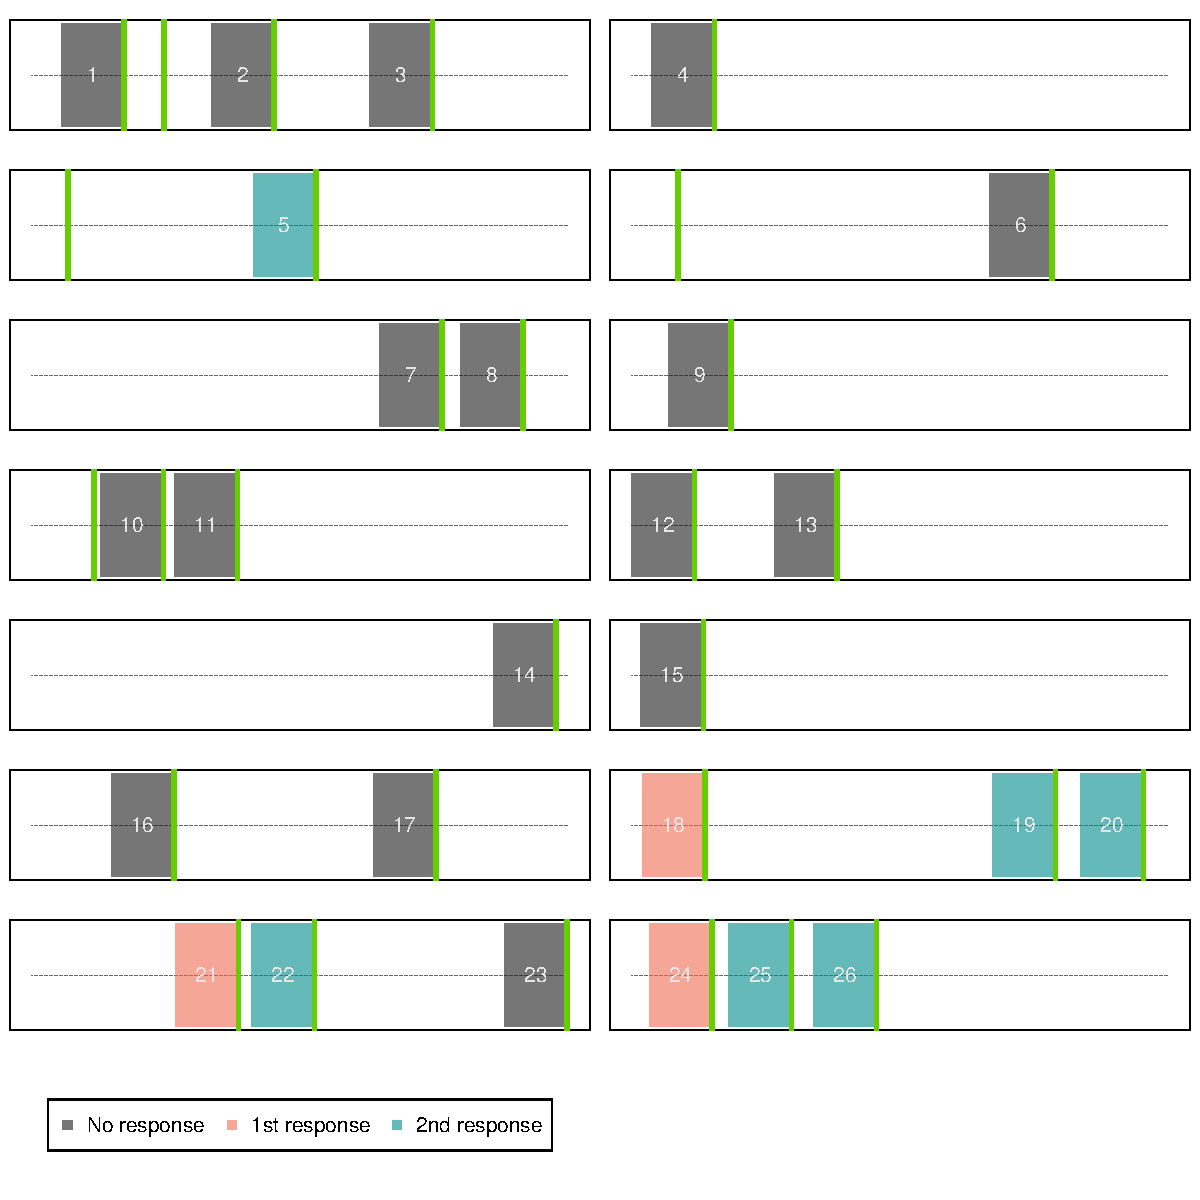
\includegraphics[width = \textwidth, keepaspectratio]{./figs/trialplot.pdf}
%   % \end{picture}
%   \end{center}
%   \label{fig:trialplot} 
%   \caption{Schematic plot of trial data. Each rectangle 
%            represents a single time period. The green 
%            vertical bars indicate applications of the stimulus.}
% \end{figure}

Data was gathered from 13 distinct time periods during which the 
stimulus was applied between one to four times. 
The 4-minute segments preceding the stimulus was used 
to predict outcomes and there were 26 trials in total.
 The result of each trial was were coded as either a seizure 
 or no seizure and we refer to a seizure as a positive response. 
Coding was based on the visible response of the 
mouse. The EEG signals around the stimulus period were also visually examined to check the accuracy of the coding.
The iEEG and LFP signals was sampled at 1220.7 Hz and
a bandpass filter removed frequencies below 0.5 Hz and greater
than 300 Hz. A notch filter was applied at 60 Hz and its harmonic frequencies. 


\section{EEG Features}

The features used to predict seizure outcomes 
 consisted of windowed spectral band power
estimates, variance, spectral entropy and the Hurst parameter.
All features were calculated on non-overlapping 2 second intervals. 
The power in frequency bands 
delta, theta, alpha, beta, and gamma was calculated 
as the integral of the spectral density $f(\lambda)$ 
computed as a smoothed periodogram. For example, 
delta band power, $\delta B$, corresponds to 
the frequency band $0.5-4Hz$ and integrates  
$f(\lambda)$ over over this interval
\[
  \delta B = \int_{0.5}^{4} f(\lambda) d\lambda. 
\]
The frequency bins corresponding to the remaining
theta, alpha, beta and gamma frequency bands are 
$ 4-8Hz, 8-12Hz, 12-30Hz, 30-100Hz$, respectively.
Band power for each interval was 
normalized by dividing by total band power on the interval

% A smaller features was selected from a group of 
% linear and non-linear features 
% based on the features ability to 
% classify the simulation groups used in Chapter 3. 
% Features that did not increase the performance of a random 
% forest classifier were omitted from the final feature set.
% The initial set of features were sample entropy, approximate entropy,permutation entropy, spectral entropy, a Hurst 
% parameter estimator, wavelet variance, a fractal dimension estimator and signal variance. Of these, variance, spectral entropy and the Hurst parameter were used in our final classifier.

%  were tested for their ability to discriminate between the same two groups of simulations used in Chapter 3 to test the approximation methods used in estimating complexity coefficients. Based on these results, spectral entropy, fractal dimension, the Hurst parameter and the wavelet coefficients, along with the spectral band power features and the complexity coefficients were computed on the EEG. In informal testing
% with a baseline classification model, the wavelet coefficients did not improve classification results and were removed from the final feature set. Given more data, feature selection might have been better performed through cross-validation on a training set. On the other hand, one of our goals was to work with a reduced feature set that was more readily interpretable. 

 \textit{Spectral entropy} is a measure of the distribution of 
 power in the spectrum of a signal. 
\[  
  SE = - \int_{-\pi}^{\pi} f(\lambda) \log f(\lambda) d \lambda.
\]
This calculation is similar to the calculation of information 
entropy where a frequency bin takes place of a discrete event.
We have defined the \textit{Hurst parameter} in Chapter 2. The Hurst 
parameter is a measure of long-range of a time series and indicates 
a slow decay in a time series autocorellation function. The Hurst parameter was estimated using the corrected empirical Hurst exponent\cite{weron2002}.  

% The variogram estimator of fractal dimension, $\hat D$ was also computed but was omitted from the final models as the feature appeared closely correlated with the complexity coefficient $B$. 

\section{Classification Procedure}

Prediction of a seizure outcome is treated as a binary classification
task with the two classes being a seizure response or no seizure response.
The classification procedure 
 takes place in three main steps: The time series is 
segmented based on one of our six partition methods, the classifier is trained on these segments, 
and new observations are assigned a class probability based on the 
weighted sum of probabilities assigned by the trained classifier. 
Classifier performance was evaluated using 5-fold cross-validation
and positive responses were evenly spread across the 
5 test sets. The full classification procedure for segmentation based on $\varepsilon-$complexity is outlined below. 

% We selected a small set of features for our classifier. 
% These included the band power of the  
% frequency bands delta, theta, alpha, beta and. 
% Spectral features need 
% to be computed over a windowed section of the time series 
% that is some multiple of the lowest frequency being computed 
% in order for the power estimates to have some statistical 
% validity. So using spectral features inherently reduces 
% the dimensionality of the data, for example, from several 
% thousand points a set of six values representing the 
% band power of some window of frequencies will be computed. 
%  Features including the 
% complexity coefficients are computed on 2 second intervals. 
% Change-points in the complexity coefficients are then 
% used to segment the features. The final predictor 
% is the mean of the features computed on each segment.
% The basic steps used are outlined below.

 %   \begin{algorithm}[!htbp]
 %    \label{alg:segmenet}
 %  \caption{Single channel segment classifier \label{alg:ecomplex}}
 %  \DontPrintSemicolon
 %  \SetAlgoLined
 %  \SetKwInOut{Input}{Input}\SetKwInOut{Output}{Output}
 %  \Input{$ \mathcal{F} $ a set of multivariate time series
 %      $\textbf{f} $ corresponding of length $N$.}
 %  \Input{$\mathcal{L}_f$ a set of labels $l_f$ for each time series 
 %  $ \textbf{f} $ }
 %  \Input{$\mathcal{X}$ a set of time series $x_f$ of length $N$ 
 %  used to partition each $\textbf{f}$.} 
 %  \Output{$\mathcal{M}$ a trained classification model.}
 %  % \tcp{initialize array}
 %   % Initialize the array epsilons $\leftarrow [0]$   \;
 %  \BlankLine 
 % \ForEach{$f$ in $\mathcal {F}$} {    
 %    % \tcp{initialize array}    
 %   Compute the change points for $\mathcal{x}_f$
 %      $p_f \leftarrow$  change_pts($\mathcal{X}_f$)
 %   Segment $f$ on change points $x_f$
 %     $\{ f \} \leftarrow f$
 %    \ForEach{$f$ in $\mathcal{F}$} {
 %      % \tcp{Compute the approximation error}
 %        Compute the approximation error \\ 
 %        $\varepsilon_{h,f} \leftarrow 
 %       \frac{1}{N}\norm{f_h - X_{h} }^2$.  \;
 %      % mse\leftarrow \varepsilon_{h,f}$
 %    } 
 %     Find minimium error over all $f$  \\
 %     epsilons$_h$ $\leftarrow \min \varepsilon_{h,f}$. \;
 %  }
 %  Fit a least squares linear model \\
 %   $A,B$ $\leftarrow$ lm(epsilons$_h$ $ \sim \{ \mathbb{S}_h \} $.) \;
 %  \end{algorithm}

\begin{enumerate}
  \item For each channel compute set of features
        including $\varepsilon-$complexity
        on regular intervals.
  \item For each channel, compute the change points 
        in the $\varepsilon-$complexity coefficients. 
  \item For each trial, segment all features using the change point 
        set computed in the previous step. 
  \item Compute the mean of each feature on the 
        segments. 
   \item Label the means of the segments 
         in a training 
         set with the label of the full time 
         series and use this set to train 
         a classifier.
  \item Compute the mean value of each feature for each segment.
   \item Train a classifier on the segmente feature meeans.
  \item  Using the held-out test set, 
         compute the class probability of each 
       segment of the test trial using the trained 
         classifier. 
  \item  For each trial the sum of the prediction probabilities of each segment, weighted by segment length, determine the final class probability.
\end{enumerate} \label{alg:segment-alg}

In the case of a uniform partition of the features, this
method is equivalent to simply using the average class probability for each segment to classify the trial.

% \subsection{Random Forest Classifier}

In theory, any single classifier or several classifiers could be used in steps 5 and 6.  For study we use a single classifier, random forest, which is known to perform well in a wide range of contexts. It has also been used in earlier studies employing the complexity coefficients as features. For pure prediction performance an  
ensemble of classifiers would likely perform better but the results 
might less interpretable.

The random forest classifier is constructed from a large number of individual decision trees. For numeric data with $d$ features, the decision trees partition the $d-$dimensional feature space into $d-$dimensional rectangles or hyperrectangles, each labeled with a class\cite{friedman2001}. Each decision tree's branches correspond to partitions of the feature space. For each branch of a decision tree, a subset of the features are chosen, restricting the decision to some subspace of the
feature space, and the division of that subspace is made in order to increase the class purity of the partition. The final prediction is based on the combined vote of the individual trees. In addition to a random selection of features, a random subset of observations are used to build each tree. This allows for an out-of-bag(OOB) estimate of the classifier 
accuracy which is calculated by classifying each observations using the set of trees which were built without seeing that observation \cite{breiman2001}.

The effect of individual features on the classification outcomes
can be less transparent for nonlinear classifiers, like random forest,
when compared to linear regression-based classifiers. However, there
are several ways to recover the variable importance for the 
classification trees in discriminating between classes. 
We report the mean variable importance of the random forest classifiers determined by the mean decrease in the 
Gini index across all branches
\cite{breiman2001}. The Gini index measures node purity increase, or 
the increase in the homogeneity of a class in a given node that 
results from division of the features space based on a particular
feature. Informally, for binary 
classification, variable importance measures how well a feature divides the feature space into partitions that contain a more class-homogeneous subset of the observations. In addition to variable importance we 
compare the difference of feature distributions for each class of EEG.

\begin{figure}[!htbp]
  \begin{center}
  % \begin{picture}(60,60)
  % ./figs/coeff-interp-simple-functions1.pdf
  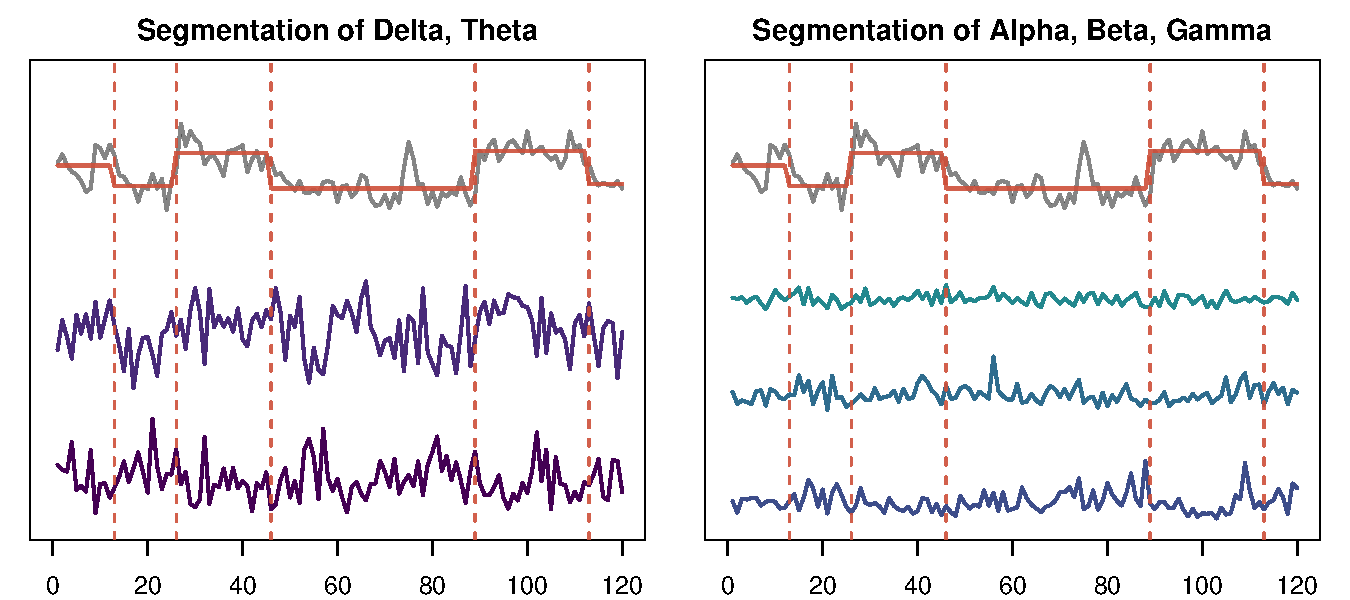
\includegraphics[width = \textwidth, keepaspectratio]{./figs/eeg-segment-plot.pdf}
  % \end{picture}
  \end{center}
  \label{fig:segplot} 
  \caption{Spectral features segmented on changes in the B complexity coefficient.}
\end{figure}

\section{Model Performance}

We begin by defining several terms we will be using to describe classifier performance. We term a seizure a 
positive response or simply a response. A  
\textit{true positive}  
is an accurate prediction of a seizure while a 
 \textit{true negative} is an accurate prediction of a non-response. 
The  \textit{sensitivity} of the classifier is then 
defined as the proportion of true positives to total 
positives
\[
  \frac{\text{True positives}}{\text{Total Positives}}
\]
 and  \textit{specificity} is the total of true 
negatives to total negatives:
\[
  \frac{\text{True Negatives}}{\text{Total Negatives}}.
\] 
Because we are using a small dataset with somewhat imbalanced classes, we report balanced accuracy in place of accuracy, and we refer to this value simply as 'accuracy'.
\[
  \text{Balanced Accuracy} = \frac{\text{Sensitivity + Specificity}}{2}.
\] 
We also report AUC, or area under the ROC curve: see 
Figure \ref{fig:eegroc} for an example ROC curve from two 
of the classifiers tested. The curve is the plot 
of the sensitivity against the false positive rate or 
$1 - $specificity and a higher AUC corresponds to a better performing classifier. An AUC of 1 indicates the correct classification of 
all observations.

A baseline classification model was built using the mean of each of the 8 features on the six channel resulting in 48 features. A random forest classifier was trained on these features and the out-of-bag classification results are reported in table \ref{tab:baseline}.
This baseline model classifies the over represented class, 
the negative or no-seizure responses, with 93\% accuracy, but 
classification of a seizure response was no better than random.
% Asymptotically this is an unbiased estimate the error on a

 \begin{table}[!htbp] \centering 
 
\begin{tabular}{@{\extracolsep{5pt}} cccc} 
\\[-1.8ex]\hline 
\hline \\[-1.8ex] 
 & Sensitivity & Specificity & Accuracy \\ 
\hline \\[-1.8ex] 
1 & $0.544$ & $0.935$ & $0.740$ \\ 
\hline \\[-1.8ex] 
\end{tabular} 
 \caption{Classification performance of baseline classifier.} 
  \label{tab:baseline} 
\end{table} 


% \begin{table}[!htbp]
% \begin{center}
%   \begin{tabular}{ | c | c |  c|} 
%   \hline 
%  Sensitivity & Specificity  &  Accuracy  \\ \hhline{|=|=|=|}
%   0.54  &  0.94     &    0.74  \\ \hline
% \end{tabular}  
% \caption{Prediction performance for baseline classifier.}
% \label{tab:baseline}
% \end{center}
% \end{table}

We compared six models to this baseline model. For each 
model a different partition scheme was used. For the models
using complexity coefficients we label the models $A, B, A+B$,
 where the label corresponds to the complexity coefficient 
 or coefficients whose change points determined the
 partition. For example, the $A + B$ model partitions
 features based on the union 
of the change points of both complexity coefficients $A$ and 
$B$. 
For three other models we partitioned features into regular 
segments of length $8, 15$ or $30$. We refer to these models
by the number of partitions.

The performance of these models was assessed using 
5-fold cross-validation where balanced sets were used for the hold-out set for each fold. The reported results are based on 50 bootstrap samples and the confidence intervals give the empirical 95\% bootstrap 
confidence intervals for each metric.
In general, all models performed best on the LFP channels, 
here labeled channel 1 and 2. The best performing model was model $8$ followed by the $B$ model.

\begin{figure}[!htbp]
  \begin{center}
  % \begin{picture}(60,60)
  % ./figs/coeff-interp-simple-functions1.pdf
  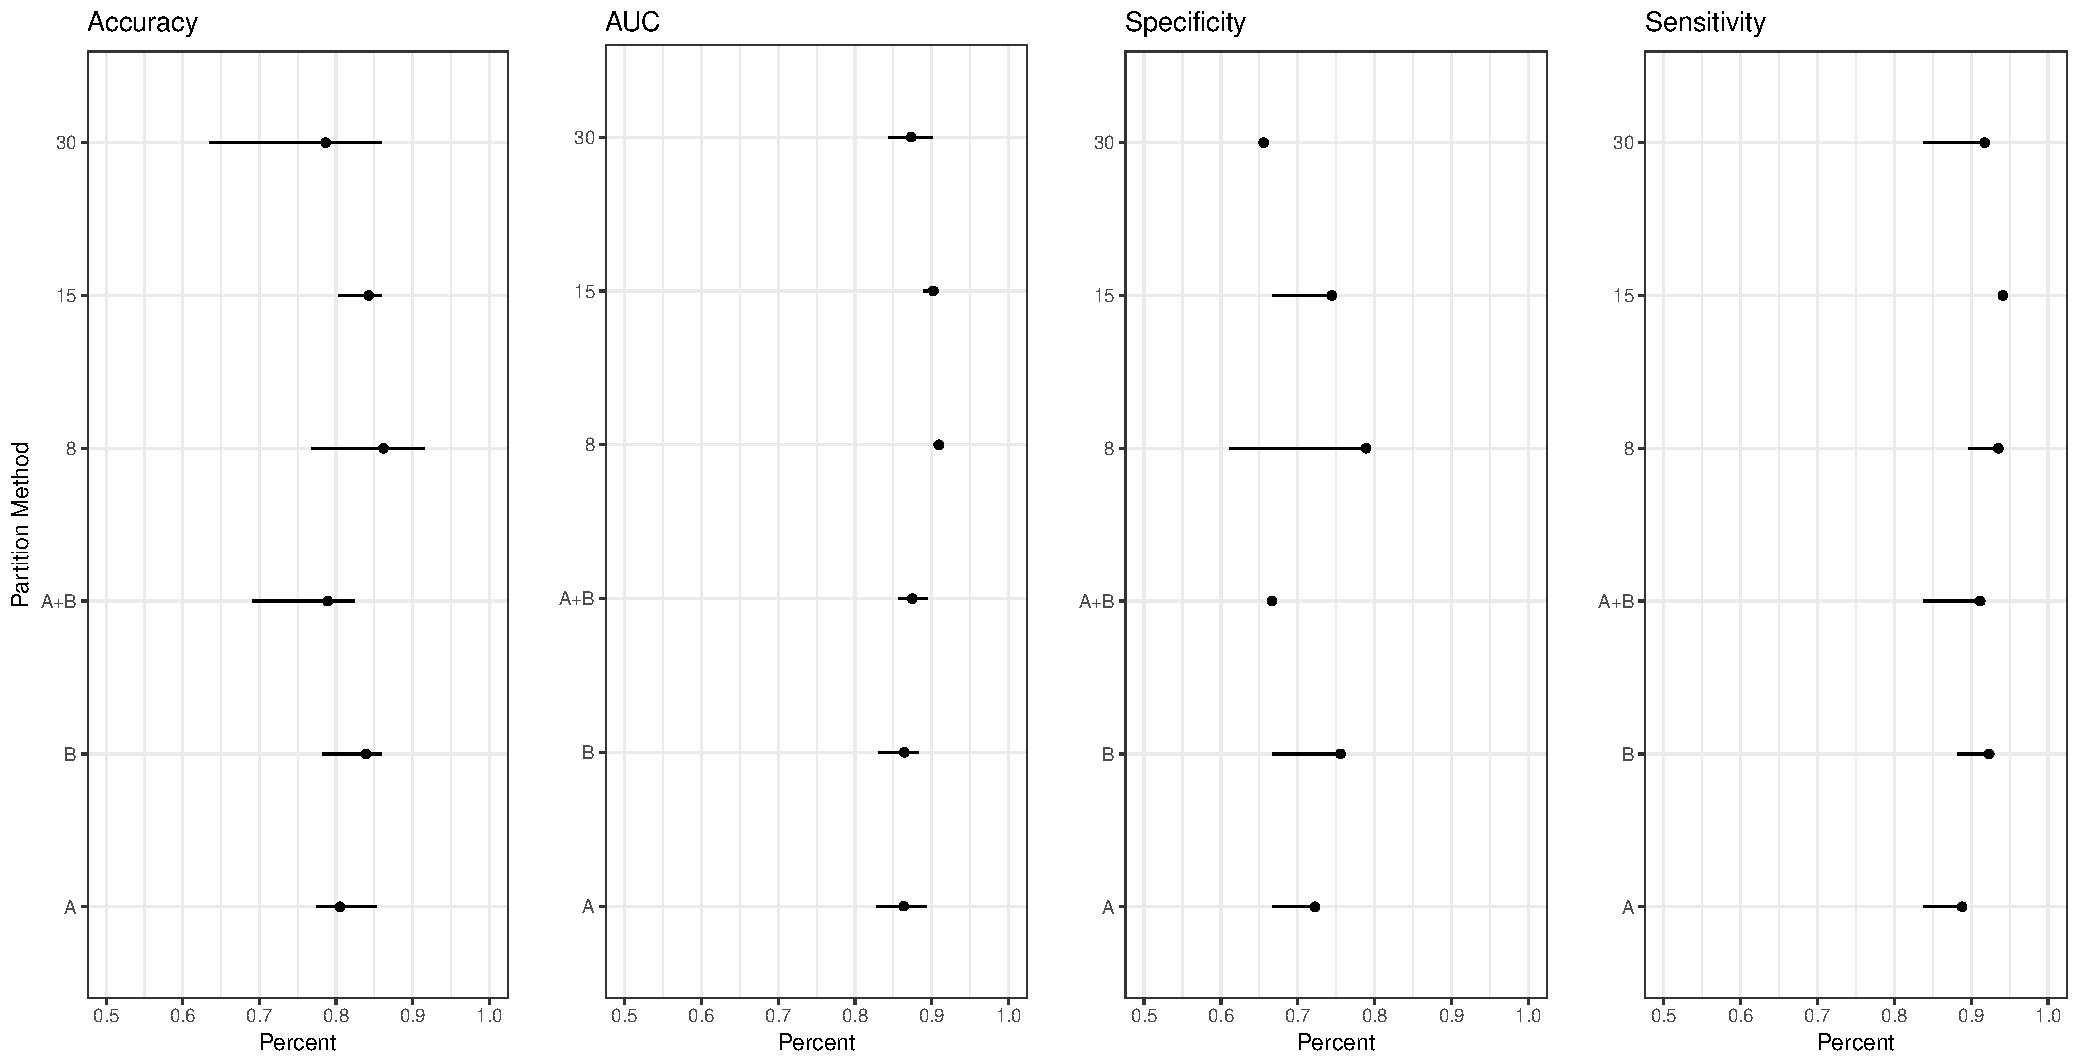
\includegraphics[width = \textwidth, keepaspectratio]{./figs/eeg-partition-diagnostic.pdf}
  % \end{picture}
  \end{center}
  \caption{Diagnostic values with 95\% bootstrap confidence intervals for each classifier trained on channel 1 features.}
  \label{fig:eeg-diagnostic} 
\end{figure}

The mean and 95\% confidence intervals for the 
performance measures for each classifier using features
computed on channel are shown in Figure \ref{fig:eeg-diagnostic}.
All methods classified non-response trials well but the two better performing
 models \textemdash model 8  and model $B$ \textemdash 
had relatively high accuracy in classifying seizure responses: 76\% for model $B$ and 79\% for model 8. 

% Table created by stargazer v.5.2 by Marek Hlavac, Harvard Unaiversity. E-mail: hlavac at fas.harvard.edu
% Date and time: Tue, Jul 11, 2017 - 02:07:16 AM
\begin{table}[!htbp] \centering 
\begin{tabular}{@{\extracolsep{-5pt}} ccccccccccccc} 
\\[-1.8ex]\hline 
\hline \\[-1.8ex] 
 & CH1 & (sd1) & CH2 & (sd2) & CH3 & (sd3) & CH4 & (sd4) & CH5 & (sd5) & CH6 & (sd6) \\ 
\hline \\[-1.8ex] 
A & 0.82 & (0.04) & 0.77 & (0.04) & 0.69 & (0.02) & 0.71 & (0.04) & 0.57 & (0.04) & 0.63 & (0.03) \\ 
B & 0.83 & (0.03) & 0.77 & (0.04) & 0.71 & (0.03) & 0.71 & (0.03) & 0.61 & (0.05) & 0.65 & (0.06) \\ 
A+B & 0.81 & (0.03) & 0.73 & (0.03) & 0.70 & (0.04) & 0.72 & (0.03) & 0.57 & (0.09) & 0.63 & (0.07) \\ 
8 & 0.83 & (0.05) & 0.82 & (0.04) & 0.74 & (0.04) & 0.72 & (0.02) & 0.75 & (0.05) & 0.74 & (0.06) \\ 
15 & 0.82 & (0.05) & 0.84 & (0.04) & 0.73 & (0.04) & 0.73 & (0.02) & 0.77 & (0.05) & 0.78 & (0.06) \\ 
30 & 0.79 & (0.07) & 0.77 & (0.05) & 0.76 & (0.04) & 0.76 & (0.03) & 0.73 & (0.08) & 0.75 & (0.04) \\ 
\hline \\[-1.8ex] 
\end{tabular} 
  \caption{Mean and standard deviation of balanced accuracy for all models.} 
  \label{tab:all-accuracy} 
\end{table} 
% Table created by stargazer v.5.2 by Marek Hlavac, Harvard University. E-mail: hlavac at fas.harvard.edu
% Date and time: Tue, Jul 11, 2017 - 02:06:02 AM
\begin{table}[!htbp] \centering 
\begin{tabular}{@{\extracolsep{-5pt}} ccccccccccccc} 
\\[-1.8ex]\hline 
\hline \\[-1.8ex] 
 & CH1 & (sd1) & CH2 & (sd2) & CH3 & (sd3) & CH4 & (sd4) & CH5 & (sd5) & CH6 & (sd6) \\ 
\hline \\[-1.8ex] 
A & 0.73 & (0.06) & 0.60 & (0.08) & 0.46 & (0.04) & 0.52 & (0.05) & 0.26 & (0.07) & 0.33 & (0.05) \\ 
B & 0.76 & (0.07) & 0.59 & (0.07) & 0.51 & (0.06) & 0.53 & (0.05) & 0.37 & (0.09) & 0.38 & (0.11) \\ 
A+B & 0.69 & (0.07) & 0.51 & (0.06) & 0.49 & (0.08) & 0.53 & (0.05) & 0.23 & (0.17) & 0.32 & (0.12) \\ 
8 & 0.77 & (0.11) & 0.70 & (0.07) & 0.59 & (0.07) & 0.54 & (0.04) & 0.62 & (0.11) & 0.57 & (0.11) \\ 
15 & 0.71 & (0.09) & 0.73 & (0.08) & 0.57 & (0.06) & 0.56 & (0.00) & 0.68 & (0.12) & 0.62 & (0.12) \\ 
30 & 0.64 & (0.14) & 0.60 & (0.09) & 0.60& (0.08) & 0.61 & (0.06) & 0.59 & (0.15) & 0.58 & (0.09) \\ 
\hline \\[-1.8ex] 
\end{tabular} 
  \caption{Mean and standard deviation of specificity for all models.} 
  \label{tab:all-specificity} 
\end{table}


The balanced accuracy of all models for each channel is
reported in Table \ref{tab:all-accuracy}. All partition
schemes resulted in fairly high rates of accuracy for channels 1 and 2. The models with a higher number of 
partitions performed significantly better on the 
iEEG channels 3-6. Accurate classification of seizures tailed off sharply for all iEEG channels as seen in Table \ref{tab:all-specificity}. In particular, specificity was greater than 70\% for only 
a few models, all of which used channels 1 or 2. The ROC and smoothed ROC curves in Figure \ref{fig:eegroc}
for are similar for both the model $A + B$ and model $8$. 


\begin{figure}[!htbp]
  \begin{center}
  % \begin{picture}(60,60)
  % ./figs/coeff-interp-simple-functions1.pdf
  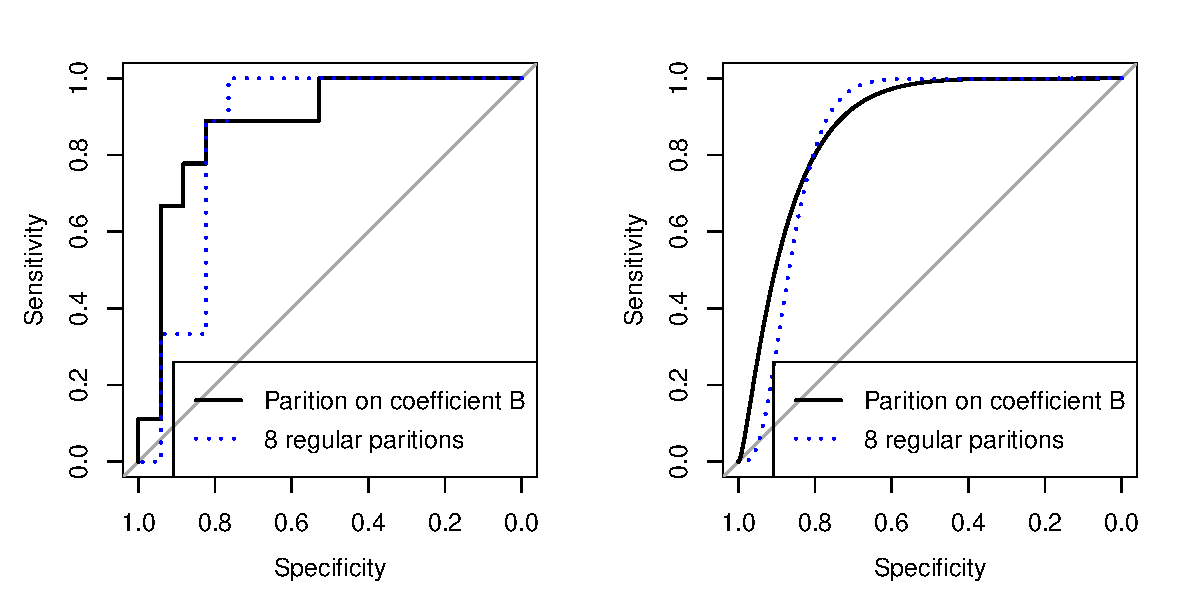
\includegraphics[width = \textwidth, keepaspectratio]{./figs/eegroc-comb.pdf}
  % \end{picture}
  \end{center}
  \caption{Best ROC curves for classifiers $B$ and $8$. On the right is the smoothed curve.}
\end{figure}
\label{fig:eegroc} 




\section{Feature Importance}

% \begin{table}[!htbp]
% \begin{center}
%   \begin{tabular}{ | c | c |  c| c | c | c |c| } 
%   \hline 
% Channel       &     1&    2 &    3 &     4 &     5 &    6  \\ \hline
% Partition Type    &       &      &     &     &  &  \\ \hhline{|=|=|=|=|=|=|=|}
% A    & 0.81 & 0.78 & 0.69 & 0.72  & 0.57  & 0.63  \\ \hline
% B    & 0.84 & 0.77 & 0.72 & 0.70  & 0.57  & 0.65  \\ \hline
% A+B  & 0.81 & 0.74 & 0.73 & 0.72  & 0.55  & 0.60  \\ \hline
% 8    & 0.86 & 0.84 & 0.73 & 0.72  & 0.74  & 0.75  \\ \hline
% 15   & 0.85 & 0.81 & 0.74 & 0.73  & 0.75  & 0.75  \\ \hline
% 30   & 0.79 & 0.75 & 0.76 & 0.77  & 0.72  & 0.77  \\ \hline
%       \end{tabular}  
% \caption{Balanced classification accuracy for each partition method 
%          and each channel.}
% \label{tab:error-allch}
% \end{center}
% \end{table}

% Table created by stargazer v.5.2 by Marek Hlavac, Harvard University. E-mail: hlavac at fas.harvard.edu
% Date and time: Sun, Jun 25, 2017 - 10:27:00 PM
 

The classification results show that seizures could be 
predicted with 
a relatively high degree of accuracy for some model 
and channel combinations. The baseline 
model aside, each of these models used features calculated 
on individual channels. This allows us to look at 
the combination of feature and channel 
associated with accurate predictions. Here 
we compare the variable importance of the more successful 
models to the difference in feature distributions 
between trials with a seizure and non-seizure response.
Random forests build multiple decision trees that divide up the feature space in complex ways and the final classification is
tallied from the votes of individual trees. This means there 
may be no clear relation between feature distribution and 
random forest variable importance. We found, however, that 
features associated with the best predictors were also associated
with clear differences in distributions between trial classes.

%  in particular 
% the features trained on predictors trained on the LFP channels 1 and 2. 

\begin{figure}[h]
  \begin{subfigure}[b]{0.45\textwidth}
      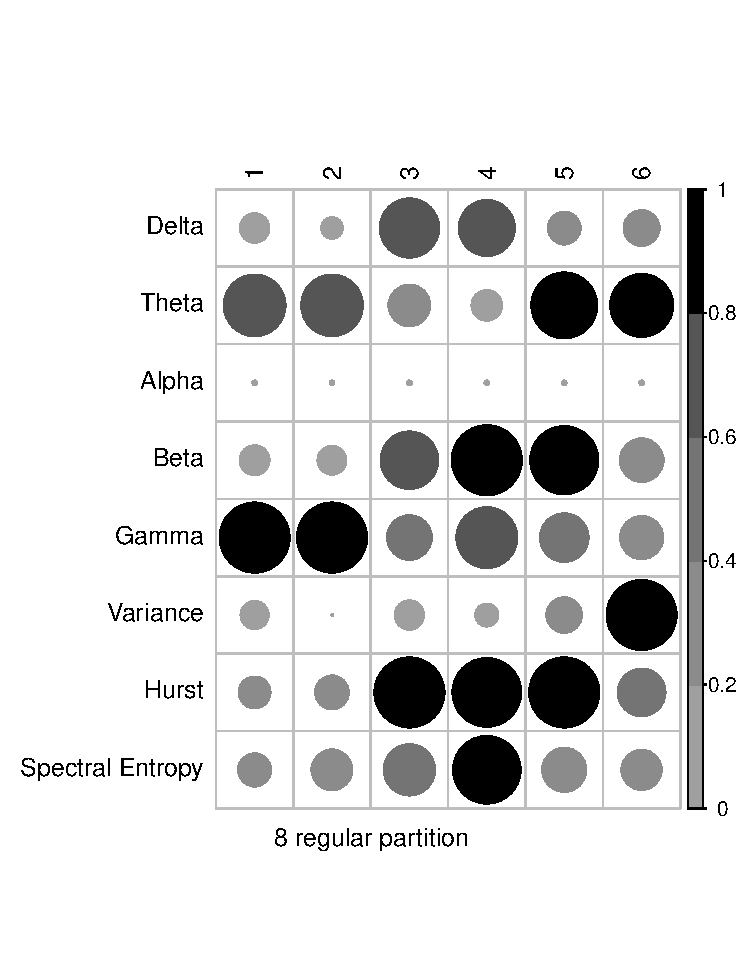
\includegraphics[width = \linewidth, keepaspectratio]{./figs/eeg-vec-corrplot.pdf}% \end{picture}
    % \caption{Functions without added noise.}
    % \label{fig:corrplot}
  \end{subfigure} 
  \hfill
  \begin{subfigure}[b]{0.45\textwidth}
    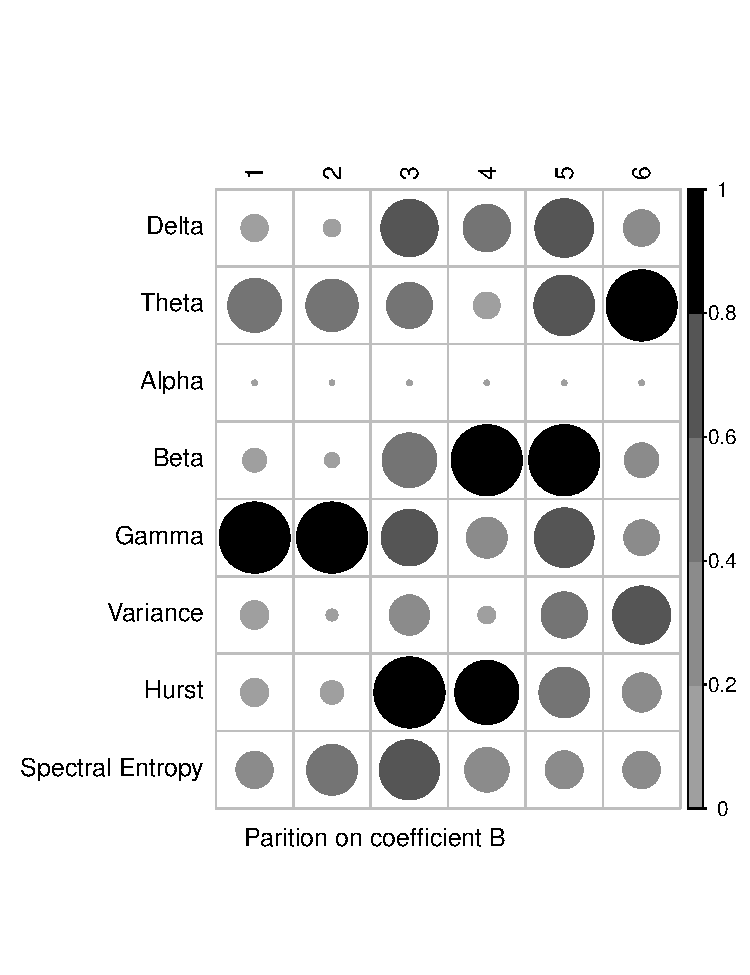
\includegraphics[width = \linewidth, keepaspectratio]{./figs/eeg-AB-corrplot.pdf}% \end{picture}
  % 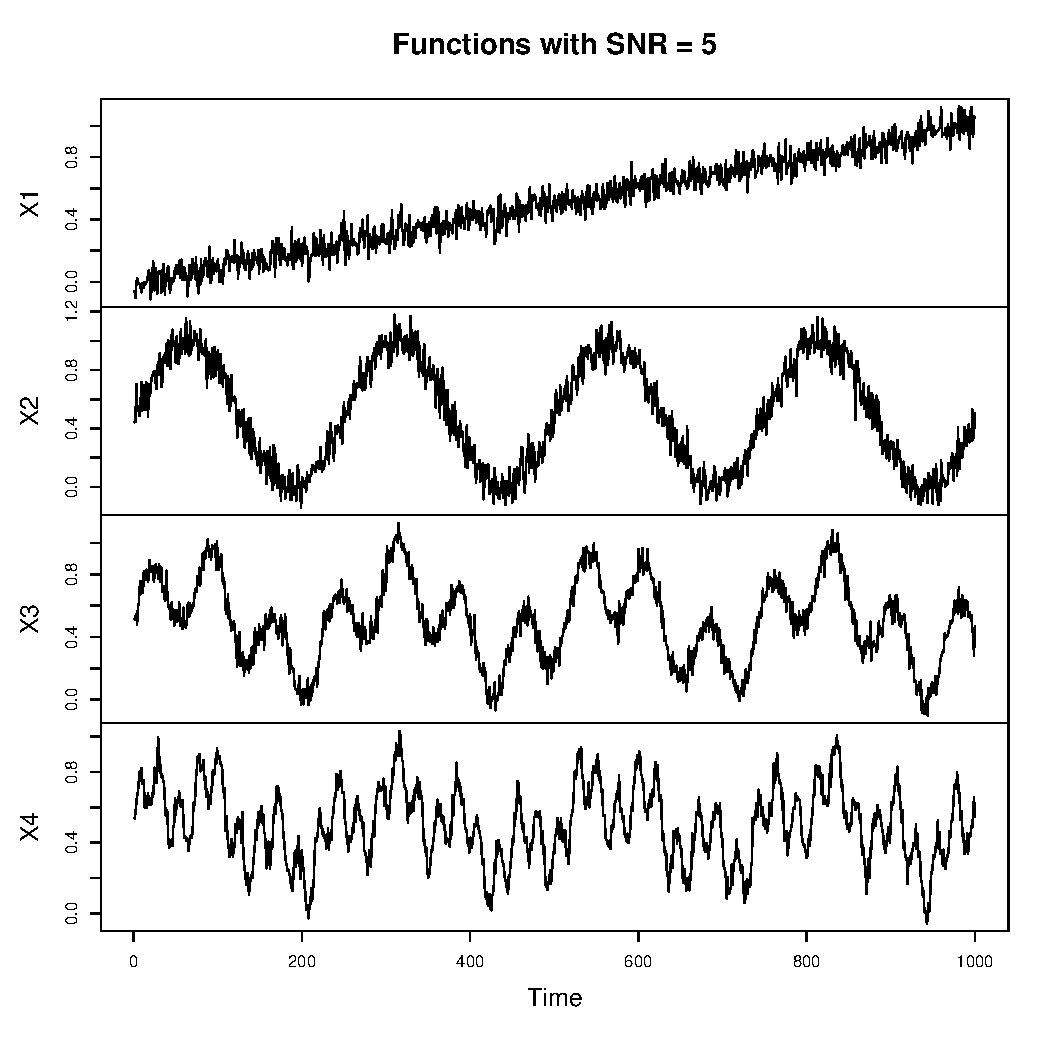
\includegraphics[width = 0.9\linewidth, height = 3in]{./figs/coeff-interp-simple-functions1.pdf}
    % \caption{Functions without added noise.}
      \end{subfigure}
  \caption{Normalized variable importance for
     each partition method and channel.}
    \label{fig:corrplot}
\end{figure}

In Figure \ref{fig:corrplot} we show the variable 
importance for the two best performing models $B$ and the 
model $8$. We have normalized variable importance to a $[0,1]$ interval for each model and
channel so the figure shows the relative importance of the variable for each model. There is a common pattern in the variable importance across the two models. Gamma and theta power had the greatest importance for the best performing models, those trained on the LFP channels 1 and 2. Both partition methods also show increased importance for beta on channels 4 and 5 and increase the importance of the Hurst coefficient for channels 3 and 4. However, no model 
was able to accurately predict seizures using these channels 
in isolation. The maximum specificty among all models trained 
on these channels was 68\% and for the two models depicted 
in \ref{fig:corrplot} this number was 59\%. 

\begin{figure}[!htbp]
  \begin{subfigure}[b]{ \textwidth}
  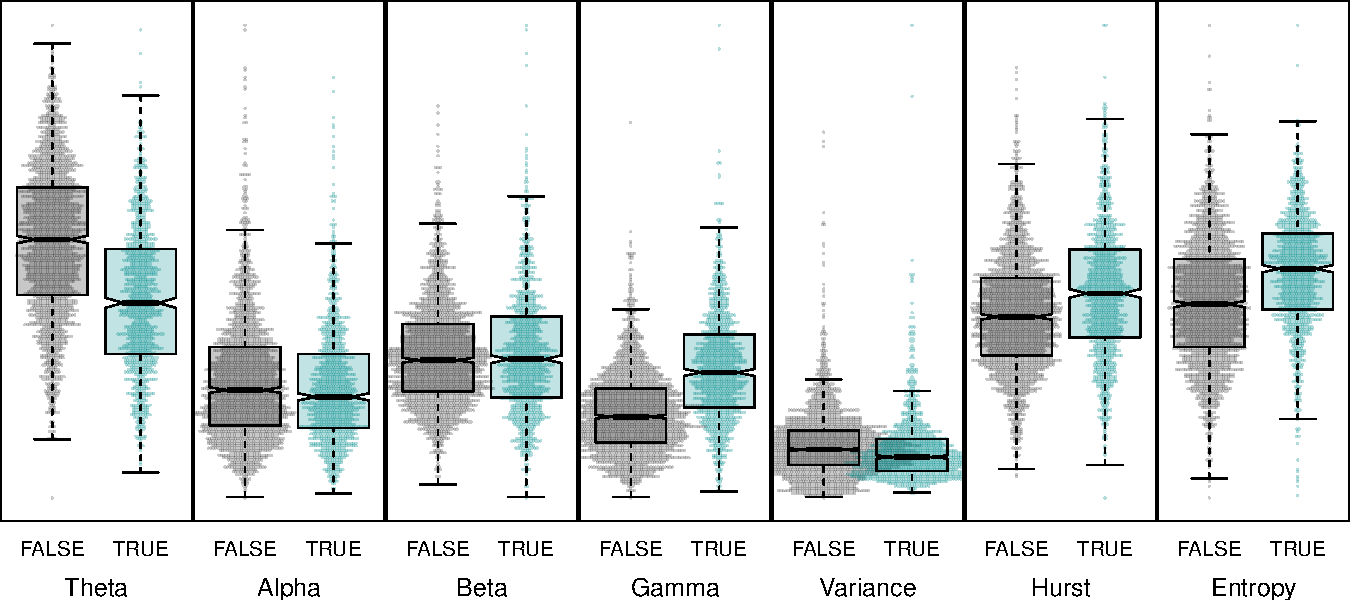
\includegraphics[width = \textwidth, keepaspectratio]{./figs/eeg-boxplot1.pdf}
    % \label{fig:corrplot}
  \end{subfigure} 
  \hfill
  \begin{subfigure}[b]{\textwidth}
  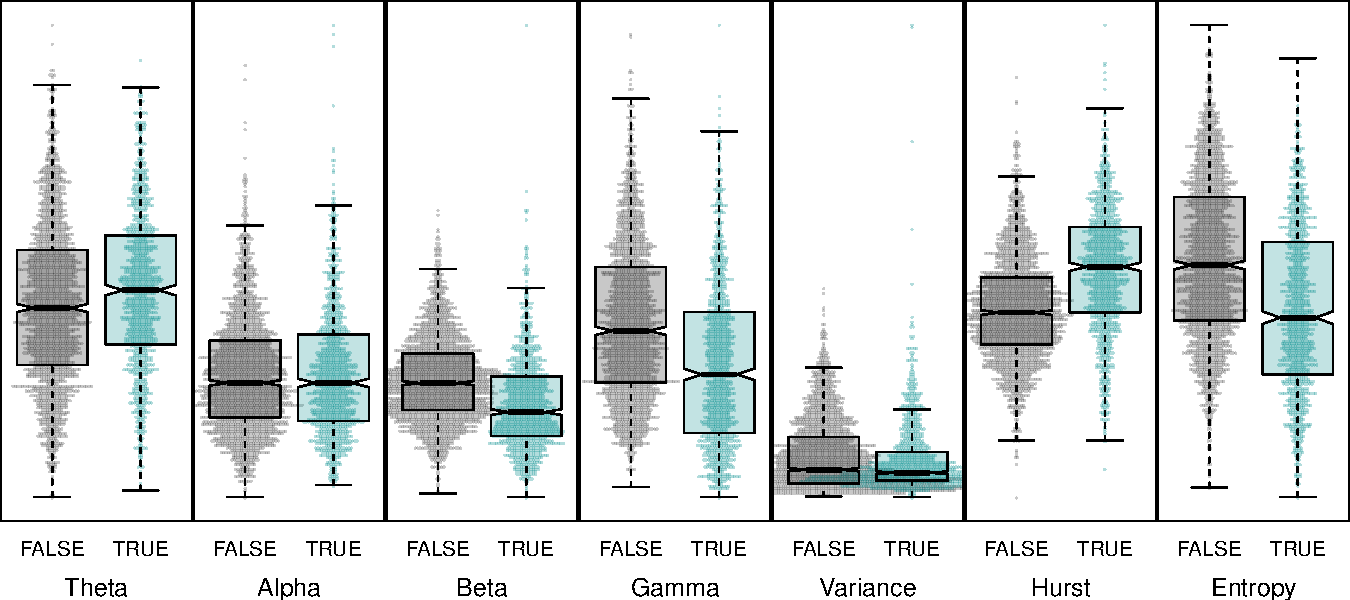
\includegraphics[width = \textwidth, keepaspectratio]{./figs/eeg-boxplotch3.pdf}
  % 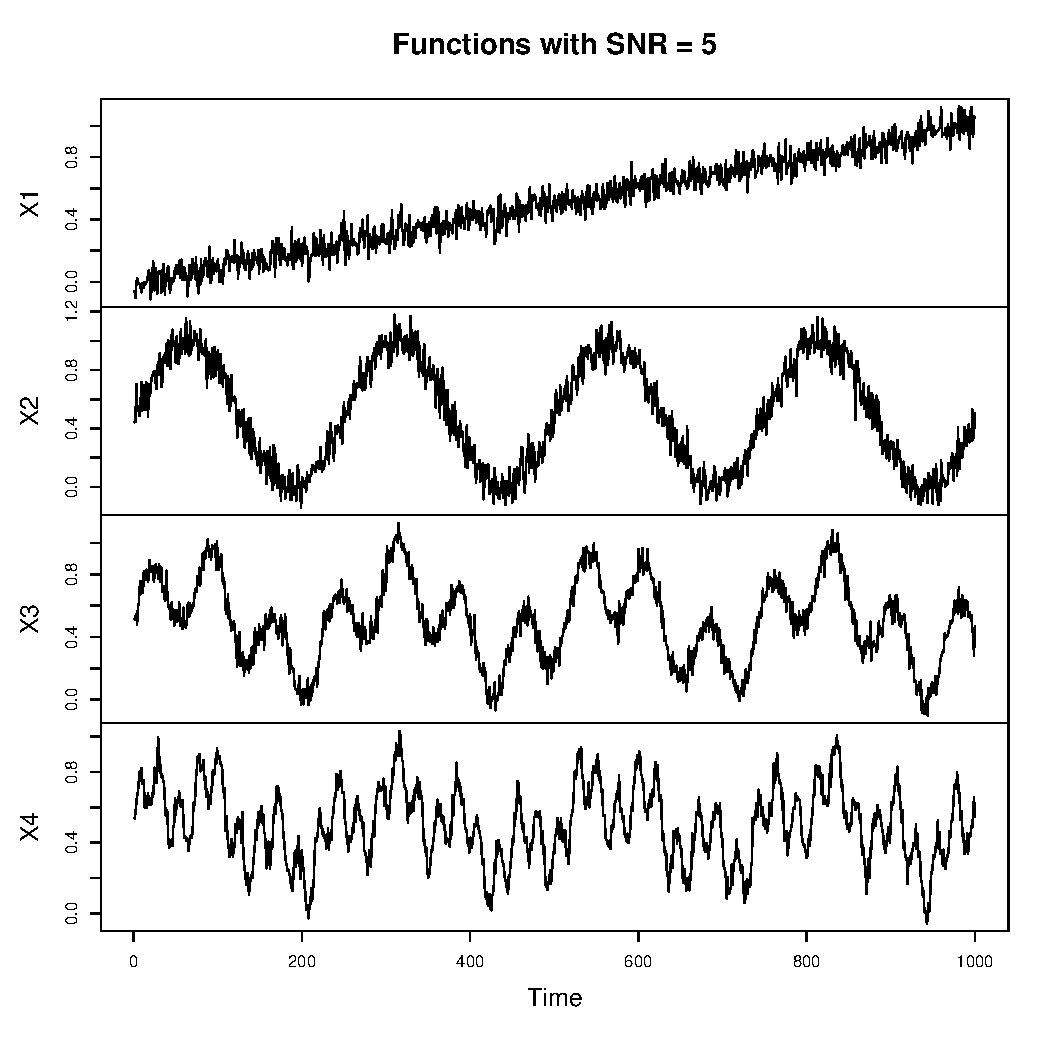
\includegraphics[width = 0.9\linewidth, height = 3in]{./figs/coeff-interp-simple-functions1.pdf}
    % \caption{Functions without added noise.}
      \end{subfigure}
  \caption{Feature distribution for channels 1(top) and 3(bottom).}
  \label{fig:boxplot}
\end{figure}

% \begin{figure}[!htbp]
%   \begin{center}
%   % \begin{picture}(60,60)
%   % ./figs/coeff-interp-simple-functions1.pdf
%   % \end{picture}
%   \end{center}
%   \label{fig:eegroc} 
%   \caption{Feature distribution for channel 1.}
% \end{figure}

% \begin{figure}[!htbp]
%   \begin{center}
%   % \begin{picture}(60,60)
%   % ./figs/coeff-interp-simple-functions1.pdf
%   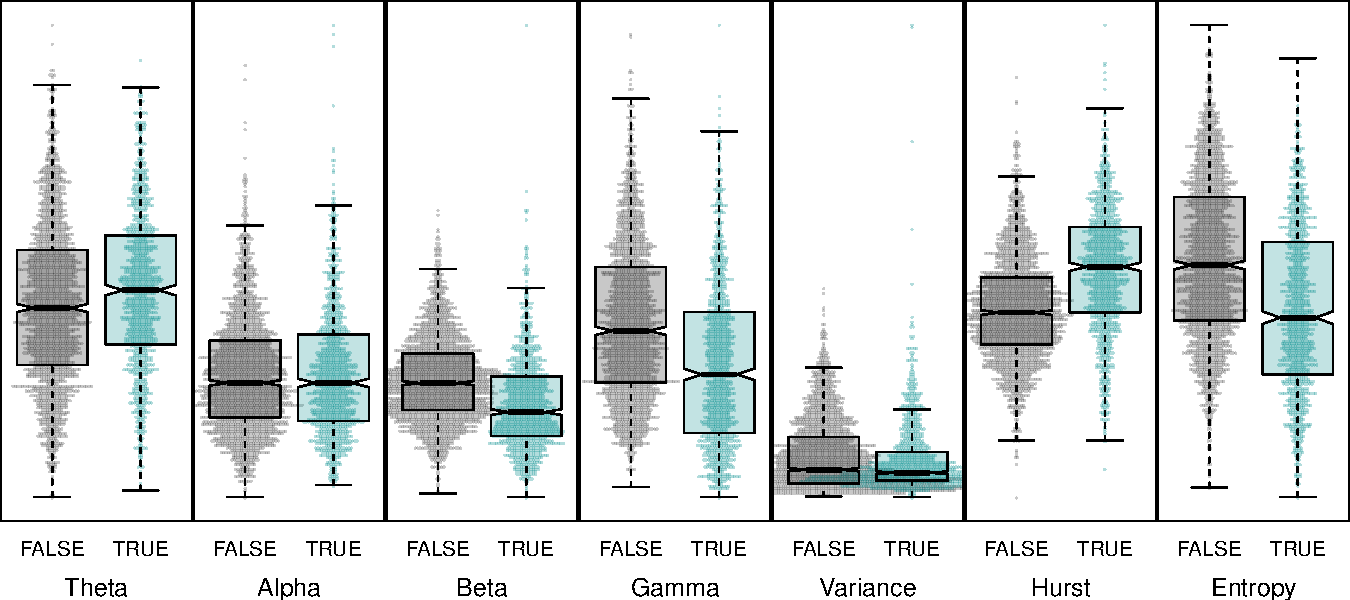
\includegraphics[width = \textwidth, keepaspectratio]{./figs/eeg-boxplotch3.pdf}
%   % \end{picture}
%   \end{center}
%   \label{fig:eegroc} 
%   \caption{Feature distribution for channel 1.}
% \end{figure}

Variable importance as measured by the random forest classifiers 
was also reflected in distributional differences in the features. 
The box plots in figure \ref{fig:boxplot} show the distribution 
and features for channels 1 and 3.  For channel 1, the relative 
power of the gamma band is higher and the power of the theta band 
was lower for trials with 
seizure responses. The median of theta and gamma power fall outside the inter-quartile range and a similar distribution was similar for channel two.  For channel three, the relative power of theta
and gamma are reversed with gamma power lower and theta power higher. 
On the other hand, the distribution of beta power for channels 1 and 2 
were similar while beta power was significantly lower for channels 3 and 4. Table \ref{tab:pvals}
shows the p-value determined by the unpaired 
Wilcoxon or Mann Whitney test, a nonparametric test for the difference 
in the location of two distributions. While the large number of data points that even small differences will be statistically significant, the table does highlight the non-significant values. 

% Table created by stargazer v.5.2 by Marek Hlavac, Harvard University. E-mail: hlavac at fas.harvard.edu
% Date and time: Mon, Jun 26, 2017 - 08:05:44 PM

\begin{table}[!ht] \centering 
\begin{tabular}{@{\extracolsep{5pt}} ccccccc} 
\\[-1.8ex]\hline 
\hline \\[-1.8ex] 
 Channel & 1 &  2 &  3 &  4 & 5 &  6 \\ 
\hline \\[-1.8ex] 
Delta & $< .0001$ & $< .0001$ & $< .0001$ & $< .0001$ & $< .0001$ & $< .0001$ \\ 
Theta & $< .0001$ & $< .0001$ & $< .0001$ & $< .0001$ & $< .0001$ & $< .0001$ \\ 
Alpha & $0.022$ & $0.699$ & $0.897$ & $0.891$ & $0.008$ & $0.302$ \\ 
Beta & $0.826$ & $0.226$ & $< .0001$ & $< .0001$ & $< .0001$ & $< .0001$ \\ 
Gamma & $< .0001$ & $< .0001$ & $< .0001$ & $< .0001$ & $< .0001$ & $< .0001$ \\ 
Variance & $< .0001$ & $< .0001$ & $0.687$ & $0.005$ & $< .0001$ & $< .0001$ \\ 
Hurst & $< .0001$ & $< .0001$ & $< .0001$ & $< .0001$ & $< .0001$ & $< .0001$ \\ 
Spectral Entropy & $< .0001$ & $< .0001$ & $< .0001$ & $< .0001$ & $0.0003$ & $< .0001$ \\ 
\hline \\[-1.8ex] 
\end{tabular} 
  \caption{Results of an unparied Wilcoxon test.} 
  \label{tab:pvals} 
\end{table} 

We report the difference of medians in \ref{median-dff}. For each feature and channel the feature values were normalized to $(0,1)$. The table 
represents the difference of medians of each feach after features ranges
were normalized to a $[0,1]$ interval. The value is the difference 
\[
  \text{Seizure median} - \text{Non-seizure median}
\]
for each feature and channel.


% Table created by stargazer v.5.2 by Marek Hlavac, Harvard University. E-mail: hlavac at fas.harvard.edu
% Date and time: Wed, Aug 09, 2017 - 04:46:01 PM
\begin{table}[!htbp] \centering 
\begin{tabular}{@{\extracolsep{-5pt}} ccccccc} 
\\[-1.8ex]\hline 
\hline \\[-1.8ex] 
 & Channel 1 & Channel 2 & Channel 3 & Channel 4 & Channel 5 & Channel 6 \\ 
\hline \\[-1.8ex] 
Delta & $0.04$ & $0.03$ & $0.05$ & $0.05$ & $0.03$ & $0.03$ \\ 
Theta & $$-$0.09$ & $$-$0.09$ & $0.02$ & $0.02$ & $$-$0.05$ & $$-$0.06$ \\ 
Alpha & $$-$0.01$ & $0$ & $0$ & $0$ & $$-$0.01$ & $0$ \\ 
Beta & $0$ & $0$ & $$-$0.04$ & $$-$0.04$ & $$-$0.02$ & $$-$0.01$ \\ 
Gamma & $0.05$ & $0.05$ & $$-$0.05$ & $$-$0.05$ & $0.05$ & $0.04$ \\ 
Variance & $0$ & $0$ & $0$ & $0$ & $0$ & $0$ \\ 
Hurst & $0.01$ & $0.01$ & $0.02$ & $0.02$ & $0.01$ & $0.01$ \\ 
Spec. Entropy & $0.02$ & $0.02$ & $$-$0.04$ & $$-$0.04$ & $0.01$ & $0.01$ \\ 
\hline \\[-1.8ex] 
\end{tabular}
\caption{Normalized difference of medians (Seizure $-$ Non-seizure) for each feature and trial.} 
  \label{median-diff}  
\end{table} 
 

% % Table created by stargazer v.5.2 by Marek Hlavac, Harvard University. E-mail: hlavac at fas.harvard.edu
% % Date and time: Tue, Aug 08, 2017 - 03:18:55 PM
% \begin{table}[!htbp] \centering 
%   \caption{} 
%   \label{} 
% \begin{tabular}{@{\extracolsep{-5pt}} ccccccccc} 
% \\[-1.8ex]\hline 
% \hline \\[-1.8ex] 
%  & Delta & Theta & Alpha & Beta & Gamma & Variance & Hurst & Spec. Entropy \\ 
% \hline \\[-1.8ex] 
% Channel 1 & $0.04$ & $$-$0.09$ & $$-$0.01$ & $0$ & $0.05$ & $0$ & $0.01$ & $0.02$ \\ 
% Channel 2 & $0.03$ & $$-$0.09$ & $0$ & $0$ & $0.05$ & $0$ & $0.01$ & $0.02$ \\ 
% Channel 3 & $0.05$ & $0.02$ & $0$ & $$-$0.04$ & $$-$0.05$ & $0$ & $0.02$ & $$-$0.04$ \\ 
% Channel 4 & $0.05$ & $0.02$ & $0$ & $$-$0.04$ & $$-$0.05$ & $0$ & $0.02$ & $$-$0.04$ \\ 
% Channel 5 & $0.03$ & $$-$0.05$ & $$-$0.01$ & $$-$0.02$ & $0.05$ & $0$ & $0.01$ & $0.01$ \\ 
% Channel 6 & $0.03$ & $$-$0.06$ & $0$ & $$-$0.01$ & $0.04$ & $0$ & $0.01$ & $0.01$ \\ 
% \hline \\[-1.8ex] 
% \end{tabular} 
% \caption{Normalized difference of medians (Seizure - Non Seizure) for each feature and trial.} 
%   \label{median-diff} 
% \end{table} 

While we were able to predict a seizure result 
with relatively high accuracy for several segmentation models,
there are some 
limitations to the study. Data from 4 mice  
were used in the experiments but the 
trials resulting in seizures came from a single mouse. 
Data from trials with seizure repsonses for additional 
mice would be 
required to know whether the features associated 
with seizures migth hold more generally. In addition, 
most of the seizures 
came from stimuli applied within two trials. 
Several of the seizures responses, then, 
occurred after a previous seizure. 
Therefore, features found predictive of a seizure may  
be conflated with features that are a result of a seizure. 
% As mentioned in the limitations section, the seizure responses 
% came in all cases from a single mouse and most of those 
% seizures came in trial periods during which there was more than one 
% seizure. Whether the predictive model generalizes to other cases
% and whether the differences in features that were predictive of 
% a seizure are similar for other subjects remains open. 
Due to the small number of trials, we did not 
have a hold-out data set. The lab which produced the 
dataset is collecting additional data.  
Testing the predictive models described here against 
new data would better indicate whether their predictive power 
generalize well. 
% Although feature importance seemed robust to changes 
% in the partitions comparing feature performance across other 
% predictive models 
On some channels, the segmentation model based on the complexity coefficients performed as well as the models with regular partitions for some channels. However, the regular partition models performed more consistently across channels. For models trained on the iEEG electrodes, channels 3-6, those that used uniformly partitioned features performed better than those partitioned on change points in the complexity coefficients. 

Another source of possible variation in the complexity-coefficient segmentation model is the window on which $\varepsilon-$complexity is calculated. The change-point detection algorithm is sensitive to the density at which the complexity-coefficients were computed. Only two variations in the feature window were tested, one at 4 second intervals and one at 2 second intervals. The 4 second window interval resulted in too few samples to adequately test for change points in the 
complexity coefficients. The feature extraction step is the most computationally expensive, but computing both the complexity coefficients and the other features on a sliding, overlapping, window would possibly allow for a better detection of change points in the diagnostic sequence of the complexity coefficients. On average, the uniform partitions divided the trials into more segments than when the trials were
segmented based on the 
complexity coefficients. It may be that simply increasing the number 
of segments in comparison to the complexity coefficient segmentation
is what improved the consistency of the models with uniform 
partitions. 
Tests of this segmentation model on simulated data sets or a wider range of time series would be needed to assess the performance of this 
method in more general contexts.  

% One of our assumptions was that arbitrary partitioning would average over changes variations in the features that corresponded to transient states. 
% But whether the complexity coefficients capture significant
% changes in the underlying dynamics that are useful for classification might depend on both feature selection and the classification task. 

% As mentioned above, with only a small set of observations, 
% improved classification on one or two instances
% would affect the performance of the classifier.
% Whether the model used here --
% partitions based on complexity coefficients -- would be successful in other contexts remains to be seen. 






